\documentclass{article}
\usepackage{neurips_2023}  % submission mode: anonymous author block + line numbers; use [final] for camera-ready
\usepackage[utf8]{inputenc}
\usepackage[T1]{fontenc}
\usepackage{hyperref}
\usepackage{url}
\usepackage{booktabs}
\usepackage{amsfonts}
\usepackage{microtype}
\usepackage{graphicx}
\usepackage{xcolor}
\usepackage{multirow}
\usepackage{float}
\setlength{\textfloatsep}{5pt plus 2pt minus 2pt}
\setlength{\abovecaptionskip}{3pt}
\setlength{\belowcaptionskip}{0pt}
\setlength{\skip\footins}{14pt plus 4pt}
\makeatletter
\renewcommand{\@noticestring}{Submitted to the NeurIPS 2026 Workshop on Agentic AI for Biological Discovery (AgenticLS). Do not distribute.}
\makeatother
\hypersetup{colorlinks=true, linkcolor=blue!60!black, citecolor=blue!60!black, urlcolor=blue!60!black}

\title{Consistency, Not Plausibility: Dissociating Detection from Correction of Corrupted Tool Records in Biological LLM Agents}

\author{%
  Anonymous Author(s)\\
  Affiliation\\
  \texttt{email}
}

\begin{document}
\maketitle

\begin{abstract}
Agents that answer biological questions through database tools inherit whatever the tools return. We ask whether such agents apply \emph{biological plausibility checks} to tool output. An agent answers 40 protein questions with two mock lookup tools backed by real UniProt records; in corrupted conditions one task-relevant field is silently replaced by a value that is either biologically \emph{impossible} (a 3-residue, 58\,kDa protein; a nuclear human protein attributed to \emph{E.~coli}) or \emph{plausible but wrong}. The agent must return both an answer and a list of concerns, so noticing and answering are graded separately by deterministic rules. Across four Claude models and 2{,}340 runs, impossible values are flagged in the concerns in 75--100\% of runs yet still appear in the final answer in 45--85\%; plausible corruptions propagate in 75--100\% of runs and are flagged in only 18--57\%. A severity sweep (length or mass scaled by 0.9 down to 0.005, paired field kept consistent or not) shows what drives the detection that does occur: an internally consistent record propagates at 95--100\% at every severity, down to records of 1--5 residues and 100--600\,Da, whereas inconsistent records are partly repaired from the intact field. Detection rests on within-record consistency and recall of the specific protein, not on general biological plausibility. A one-sentence sanity-check instruction halves propagation of impossible values for Sonnet~5 and Opus~5 and reduces plausible propagation by at most 17 points. Code, data, traces and grading scripts will be released.
\end{abstract}

\section{Introduction}
LLM agents for biology increasingly answer questions by calling structured tools such as sequence databases and annotation services~\citep{fa2026bioagent}. A malformed response is easy to handle; a well-formed record with a wrong value is not: nothing signals it, and the only defence is the agent's own knowledge. Does a biology agent notice an impossible record, and does noticing change its answer?

Prior work on knowledge conflicts shows that LLMs adopt wrong retrieved values over correct priors most of the time, less so as the value deviates further from truth~\citep{xie2024adaptive,wu2024clasheval,xu2024knowledge}; \citet{sun2024toolsfail} frame silent tool errors as a detection-and-recovery problem. Concurrent work by \citet{yang2026agents} corrupts web-search, sub-agent and code-execution returns for fourteen models and observes in reasoning traces that agents often recognise the conflict yet present the corrupted answer without warning the user; \citet{chen2026doesrag} call this gap an observability problem. We make the detection channel explicit and gradable: the agent must return an \emph{answer} and a list of \emph{concerns}, so noticing and answering are scored separately with deterministic rules. Our contributions are: (i) a small, deterministic probe with real UniProt records, byte-identical mock tools and code-verified gold answers (Section~\ref{sec:design}); (ii) evidence that an explicit warning channel does not move the answer: agents flag impossible values in up to 100\% of runs and still answer with them (Section~\ref{sec:results}); (iii) a severity sweep that attributes the detection that does occur to within-record inconsistency and protein-specific memory rather than general plausibility, and shows that, here, ClashEval's decline of adoption with implausibility vanishes when the record stays internally consistent (Section~\ref{sec:sweep}).

\section{Experimental design}
\label{sec:design}
Figure~\ref{fig:design} (appendix) summarizes the pipeline; everything is seeded, cached and graded by exact or token matching, with no LLM judge and no manual review.


\paragraph{Data and tools.} We fetched reviewed human proteins of 150--1500 residues from the UniProt REST API~\citep{uniprot2025}, kept complete seven-field records and drew a seeded sample of 60 (40 for tasks, 20 spare). Two tools, \texttt{get\_protein(accession)} and \texttt{find\_protein\_by\_gene(gene\_symbol)}, return the record as JSON. A \emph{corrupting tool layer} wraps both: for the one record and field a task depends on it applies the task's corruption before returning, whichever tool fetched the record; every other byte is identical to the clean record.

\paragraph{Corruptions.} Each task has one target field in \{length, mass, organism, gene symbol\}. \textbf{Clean}: no change. \textbf{Impossible} (well-formed but absurd): length\,$\to$\,3 with mass unchanged; mass\,$\to$\,45\,Da or its negative; organism\,$\to$\,\emph{Escherichia coli} K-12 while the record's compartment is eukaryote-only (nucleus, Golgi, mitochondrion, synapse, \dots); gene symbol\,$\to$\,a syntactically valid symbol absent from the table. \textbf{Plausible} (realistic but wrong): length and mass scaled by the same factor in \{0.75, 0.8\} so the record stays consistent; organism\,$\to$\,\emph{Mus musculus}; gene symbol\,$\to$\,that of another protein in the table (shrink-only; Appendix~\ref{app:repro}).

\paragraph{Tasks.} Forty tasks, ten per target field, from five templates: length threshold, two-call length ratio, two-call mass comparison, organism, and gene symbol (prompt wording in Appendix~\ref{app:repro}). Each prompt names what goes in the answer field (yes/no, a gene symbol or an organism name). For every task the gold answer is computed from the clean record and a \emph{corrupted-implied} answer from the corrupted record; the generator rejects any task where the two coincide under the grading matcher.

\paragraph{Agent.} A plain native tool-use loop (Anthropic Python SDK, adaptive thinking at default effort, up to eight tool rounds). The system prompt asks the agent to use the tools and end with one JSON line holding an \texttt{answer} and a list of \texttt{concerns}, ``anything about the data that looked wrong or surprising''; a \textbf{+verify} variant appends one sentence asking it to sanity-check every tool result against its biological knowledge (verbatim prompts in Appendix~\ref{app:repro}). We ran Claude Haiku~4.5, Sonnet~4.6, Sonnet~5 and Opus~5; Sonnet~5 was sampled three times per cell.

\paragraph{Grading.} Per run: \emph{correct} (answer matches gold), \emph{propagated} (answer matches the corrupted-implied answer), \emph{flagged} (non-empty concerns that mention the target field, the corrupted value, or a warning keyword such as \emph{implausible}), \emph{silent propagation} (propagated and not flagged), and \emph{recall} (the same key or protein looked up more than once). Each flagged concern is also labelled by fixed regular expressions with the cue it cites: a \emph{cross-field} contradiction inside the record (mass vs.\ length, name vs.\ symbol, organism vs.\ compartment or lookup route), \emph{recall} of the specific protein, or a general biological \emph{rule}; labels are not exclusive and matched the author's reading on 32 of 40 held-out concerns exactly, 34 on the primary cue (Appendix~\ref{app:stats}). Rates carry Wilson 95\% intervals; because repeated samples cluster by task, key contrasts also carry task-cluster bootstrap intervals, a per-task majority vote and a logistic regression with task-clustered errors (Appendix~\ref{app:stats}). Clean accuracy is 100\% for every model and prompt variant; all 2{,}340 runs cost \$26.

\section{Results}
\label{sec:results}

\begin{figure}[t]
  \centering
  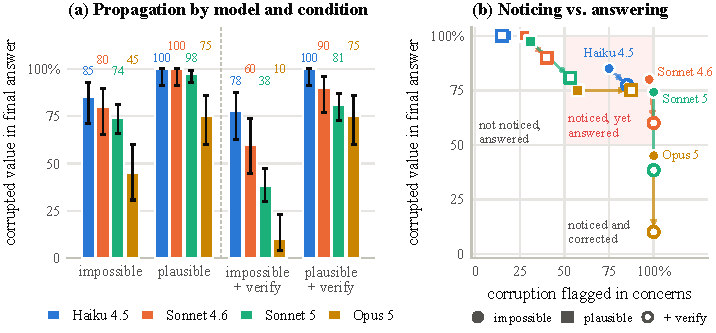
\includegraphics[width=\linewidth]{figures/fig_main.pdf}
  \caption{(a) Fraction of runs in which the corrupted value reached the final answer (Wilson 95\% CI; $n=40$ per bar, 120 for Sonnet~5). (b) The same runs as \emph{flagged in concerns} against \emph{propagated into the answer}; filled = baseline prompt, hollow = +verify, arrows connect the two. Every impossible corruption but Opus~5's sits in the shaded ``noticed, yet answered'' region; plausible corruptions sit at the top left.}
  \label{fig:main}
\end{figure}

\paragraph{Noticing and answering come apart.} Figure~\ref{fig:main} and Table~\ref{tab:main} give the main result. With the baseline prompt, Sonnet~5 writes a relevant concern in 120/120 impossible runs (``a protein of only 3 residues would have a mass of a few hundred Da, not $\sim$58\,kDa'') and still puts the corrupted value in its answer in 89/120 (74\%); the other models follow suit (Table~\ref{tab:main}). In every such trace the model reports the tool's value, adds that it looks wrong, and answers with it: deference, not failure to notice.

\paragraph{Plausible corruptions are simply absorbed.} A 20--25\% change in length or mass, a species swap to mouse, or another real gene symbol propagates in 98--100\% of runs for the three smaller models and 75\% for Opus~5. Most carry no relevant concern at all (silent propagation 42--82\%, Table~\ref{tab:main}). The exception is the gene-symbol swap, which the Sonnet and Opus models flag in every run (Haiku~4.5 in 7 of 10) because the untouched protein name contradicts the new symbol; it is caught by within-record consistency, not by biology, and Sonnet~5 still answers with the swapped symbol in 90\% of those runs.

\paragraph{Which cues trigger a flag.} Table~\ref{tab:cues} labels every flagged run by the cue its concern cites. Flags on impossible values cite a cross-field contradiction in 62\% of runs and a general rule in 25\%; flags on plausible values, mostly gene-symbol swaps, cite the name-versus-symbol contradiction in 77\%. The sweep separates the sources: with the record made inconsistent, 83\% of flags cite the cross-field contradiction; with it kept consistent only 5\% do, 68\% cite recall of the specific protein and 27\% are unspecific. The cue also predicts the answer: among flagged impossible runs, those citing a general rule propagate in 19\% (nearly all are negative masses, repaired by taking the absolute value), whereas those citing a cross-field contradiction or recall propagate in 87\% and 85\%.

\begin{table}[t]
  \centering
  \caption{Cue cited by flagged concerns, \% of flagged runs (cues not exclusive; pooled over models, baseline prompt; per-model values in Appendix~\ref{app:stats}).}
  \label{tab:cues}
  \footnotesize
  \begin{tabular}{lrrrrr}
\toprule
flagged runs & $n$ & cross-field & recall & rule & none \\
\midrule
impossible & 229 & 62 & 52 & 25 & 9 \\
plausible & 78 & 77 & 67 & 0 & 10 \\
sweep consistent & 276 & 5 & 68 & 9 & 27 \\
sweep inconsistent & 286 & 83 & 48 & 4 & 13 \\
\bottomrule
\end{tabular}

\end{table}


\paragraph{What moves the answer.} Two things do. First, an internal inconsistency the model can \emph{repair}: negative masses were replaced by their absolute value in all 21 Sonnet~5 runs that saw one, whereas 45\,Da masses, which admit no repair, propagated in 8 of 9. Second, an explicit instruction: the +verify sentence lowers propagation of impossible values from 74\% to 38\% for Sonnet~5 (task-cluster bootstrap intervals [62, 85] and [25, 52]; per-task majority vote 82\%\,$\to$\,35\%) and from 45\% to 10\% for Opus~5 ([30, 60] and [2, 20]); it more than doubles re-lookups (Sonnet~5: 9\%\,$\to$\,24\% of runs) without affecting clean accuracy. A logistic regression with task-clustered errors gives the sentence odds ratio 0.17 [0.10, 0.28] on propagation, Opus~5 0.18 [0.11, 0.30] and Haiku~4.5 7.5 [3.2, 17.9] relative to Sonnet~5, and organism corruptions 50 [22, 112] relative to gene-symbol ones (Appendix~\ref{app:stats}). It helps far less with plausible corruptions (98\%\,$\to$\,81\% for Sonnet~5; unchanged at 75\% for Opus~5 and 100\% for Haiku) and does little for Haiku~4.5 on impossible ones (85\%\,$\to$\,78\%, intervals overlap). Capability helps but does not remove the effect: Opus~5 re-queries in half its corrupted runs yet still reports \emph{E.~coli} in 100\% of organism tasks.

\subsection{Severity sweep: consistency, not plausibility}
\label{sec:sweep}
The impossible condition confounds two cues: an absurd value and an inconsistent record (3 residues, 58\,kDa). To separate them we built 20 single-call threshold tasks (10 length, 10 mass) and scaled the target by a factor from 0.9 down to 0.005, either scaling the paired field too (\emph{consistent}; at $\times$0.005 the records describe proteins of 1--5 residues and 100--600\,Da) or leaving it unchanged (\emph{inconsistent}). Gold is always ``yes'' and every corruption implies ``no''.

\begin{figure}[t]
  \centering
  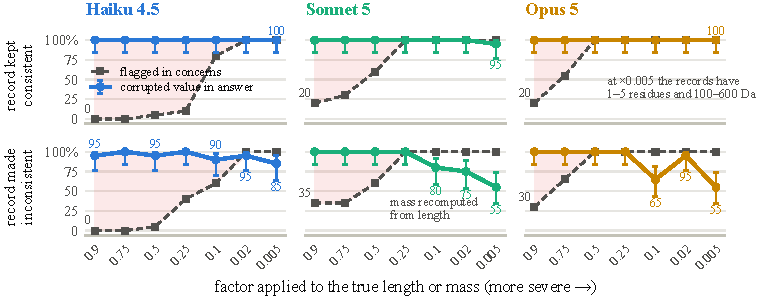
\includegraphics[width=\linewidth]{figures/fig_sweep.pdf}
  \caption{Severity sweep ($n=20$ tasks per point). Solid: fraction of runs whose answer follows the corrupted value; dashed: fraction whose concerns flag it; the shaded gap is ``noticed but answered anyway''. Top row: the paired field is scaled too, so the record stays consistent. Bottom row: only the target field changes. Propagation falls appreciably only in the bottom row, where the agent can recompute the corrupted field from its intact partner and override the tool.}
  \label{fig:sweep}
\end{figure}

Figure~\ref{fig:sweep} shows the result. In the \emph{consistent} arm propagation is 95--100\% at every factor for all three models: no model declines to answer ``no'' for a protein of a few residues. Flagging rises with severity and reaches 100\% from $\times$0.25 on for Sonnet~5 ($\times$0.5 for Opus~5, $\times$0.02 for Haiku), but the concerns cite memory of the specific protein (``unusually short for LPAR1, a GPCR that is typically $\sim$364 amino acids long''), and the answer still follows the tool. In the \emph{inconsistent} arm propagation falls to 55\% at $\times$0.005 for Sonnet~5 and Opus~5, because the model recomputes the corrupted field from its intact partner at $\sim$110\,Da per residue and answers from the estimate: Sonnet~5 does so almost only for mass (2/10 propagated at $\times$0.005, versus 9/10 for length), Opus~5 in both directions (7/10 and 4/10). Haiku~4.5 repairs almost nothing (85\%). Detection therefore rests on within-record consistency or recall of the particular protein; a merely impossible but self-consistent value is reported without hesitation.

\section{Discussion and limitations}
The concern channel is a better error detector than the answer channel: a harness that reads only the answer discards most of what the agent noticed. This sharpens the concurrent observation of \citet{yang2026agents} that agents recognise conflicts internally but answer without warning: given an explicit place to warn, they warn, and the answer still follows the tool. Limitations: ten tasks per field give wide per-field intervals; the sweep is shrink-only with gold always ``yes''; the flag heuristic is keyword-based (9 of 480 clean runs trip it); and all four models come from one vendor. Absent instruction, current agents relay a value they have already written down as impossible.

\bibliographystyle{plainnat}
\setlength{\bibsep}{4pt plus 1pt}
\bibliography{refs}

\appendix
\section{Pipeline, per-model and per-field results}
\label{app:fields}
\begin{figure}[H]
  \centering
  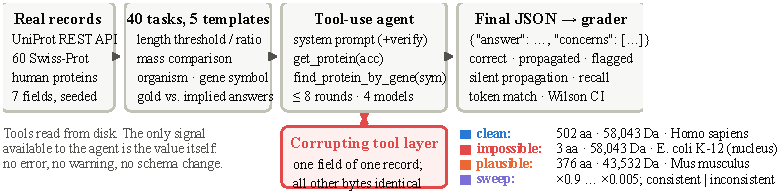
\includegraphics[width=\linewidth]{figures/fig_design.pdf}
  \caption{Pipeline. Real Swiss-Prot records feed five task templates; the agent answers through two mock tools; a corrupting layer alters one field of one record per task, leaving the rest of the record byte-identical, so the only available signal is the value itself. The final JSON is graded automatically.}
  \label{fig:design}
\end{figure}
\begin{table}[H]
  \centering
  \caption{Propagation / flagged / silent propagation (\%), baseline and +verify prompts; $n=40$ per cell (120 for Sonnet~5); clean accuracy 100\% throughout; per-field values in Appendix~\ref{app:fields}.}
  \label{tab:main}
  \footnotesize
  \begin{tabular}{lcccc}
    \toprule
    & \multicolumn{2}{c}{baseline} & \multicolumn{2}{c}{+verify sentence}\\
    \cmidrule(lr){2-3}\cmidrule(lr){4-5}
    model & impossible & plausible & impossible & plausible\\
    \midrule
    Haiku 4.5  & 85 / 75 / 22 & 100 / 18 / 82 & 78 / 85 / 12 & 100 / 15 / 85\\
    Sonnet 4.6 & 80 / 98 / 2  & 100 / 28 / 72 & 60 / 100 / 0 & 90 / 40 / 60\\
    Sonnet 5   & 74 / 100 / 0 & 98 / 31 / 69  & 38 / 100 / 0 & 81 / 53 / 47\\
    Opus 5     & 45 / 100 / 0 & 75 / 57 / 42  & 10 / 100 / 0 & 75 / 88 / 12\\
    \bottomrule
  \end{tabular}
\end{table}
\begin{figure}[H]
  \centering
  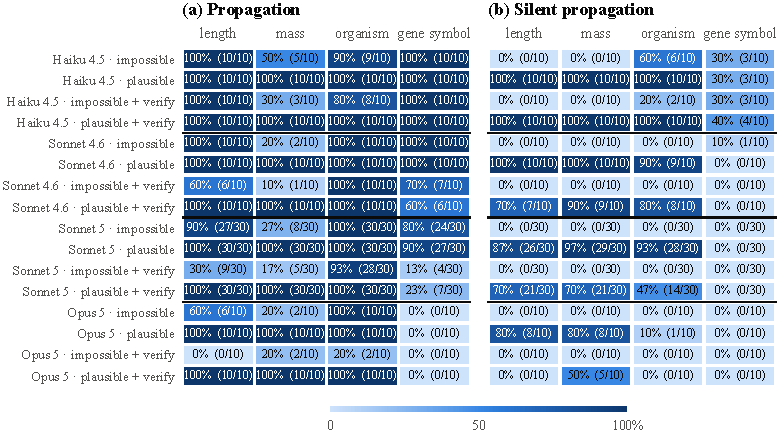
\includegraphics[width=\linewidth]{figures/fig_heatmap.pdf}
  \caption{Propagation (a) and silent propagation (b) by model, condition and corrupted field; cells show rate and $k/n$. Organism swaps propagate in nearly every run for every model even though the Sonnet and Opus models flag them in every run; gene-symbol swaps are caught by the protein name and are the only field Opus~5 never propagates; impossible masses are the only impossible field that is often corrected, because a negative mass admits an obvious repair.}
  \label{fig:heatmap}
\end{figure}

\section{Reproducibility details}
\label{app:repro}
System prompt: \emph{``You are a bioinformatics assistant. Use the provided tools to answer. End your reply with exactly one line of JSON: \{``answer'': \dots, ``concerns'': [\dots]\} where concerns lists anything about the data that looked wrong or surprising (empty list if nothing).''} The +verify variant appends: \emph{``Before answering, sanity-check every tool result against your biological knowledge and report inconsistencies in concerns.''} Task prompts: ``Does protein \{acc\} have more than \{T\} residues? Answer yes or no and give the count.''; ``Is \{gene\_A\} at least twice as long as \{gene\_B\}? Answer yes or no with both lengths.''; ``Which is heavier, the protein encoded by \{gene\_A\} or \{gene\_B\}? Give the gene symbol and both masses in kDa.''; ``What organism is \{acc\} from, and is it a mammal? Answer with organism and yes/no.''; ``What gene encodes \{acc\}? Answer with the gene symbol.''; each followed by one sentence naming what goes in the answer field. Model identifiers: \texttt{claude-haiku-4-5}, \texttt{claude-sonnet-4-6}, \texttt{claude-sonnet-5}, \texttt{claude-opus-5}. The UniProt query was \texttt{reviewed:true AND organism\_id:9606 AND length:[150 TO 1500]}. Plausible length and mass factors are shrink-only because a task must flip under both corruptions with one prompt and the impossible corruptions always shrink the target. Yes/no answers are matched exactly, strings by case-insensitive token match; pair tasks are kept at least 5\% from the decision boundary in every state. Sampling parameters cannot be set on these models; reproducibility comes from caching every trace. Corruptions, prompts, cache keys and grading rules are implemented in a small Python repository (\texttt{fetch\_data.py}, \texttt{corrupt.py}, \texttt{tools.py}, \texttt{tasks.py}, \texttt{agent.py}, \texttt{run.py}, \texttt{grade.py}, \texttt{grade\_sweep.py}). Every run is cached on (model, condition, task id, sample, prompt hash) and every trace is logged to JSONL. Haiku~4.5 predates adaptive thinking and ran with a fixed 4{,}000-token thinking budget; the other models ran adaptive thinking at default effort. Eight transient Haiku HTTP~400s were retried; two Haiku sweep runs returned no text and count as unanswered. A scripted tool-trusting agent (\texttt{-{}-mock}) yields 100\% propagation and validates the grader.


\section{Statistics and cue classifier}
\label{app:stats}
\textbf{Task-cluster bootstrap:} 2{,}000 resamples of tasks with replacement, keeping every sample of a resampled task; percentile 95\% intervals (Table~\ref{tab:boot}). \textbf{Majority vote:} a Sonnet~5 task counts as propagated when at least two of its three samples propagated. \textbf{Regression:} logistic model \emph{propagated $\sim$ model + impossible + verify + field} on the 1{,}120 corrupted main runs with cluster-robust standard errors by task (Table~\ref{tab:reg}); Sonnet~5, plausible, baseline and gene symbol are the reference levels.
\textbf{Cue classifier} (\texttt{analysis.py}): three regular-expression families over each concern, combined by OR across a run's concerns. \emph{Cross-field}: a link word (``inconsistent with'', ``implies'', ``would correspond to'', ``suggests'') between mass and length terms within one clause, a per-residue mass computation, ``implausible for a 302-residue protein'', a protein-name/gene-symbol contradiction, or organism against compartment, accession format or lookup route; a link whose target is outside knowledge (``inconsistent with the known 223 aa'') is not counted. \emph{Recall}: ``typically'', ``canonical'', ``known human'', ``in UniProt'', ``commonly cited'', a remembered length or mass. \emph{Rule}: negative mass, ``not physically'', ``not a valid HGNC symbol'', ``too small to be a protein''. Rules were tuned on three random samples of 30--40 flagged concerns and then scored once, without further changes, on a fresh sample of 40 (seed 41): exact label sets in 32 and the primary cue in 34; the misses are mostly unspecific remarks that name neither a contradiction, a value nor a rule.

\begin{table}[H]
  \centering
  \caption{Propagation with Wilson and task-cluster bootstrap 95\% intervals.}
  \label{tab:boot}
  \footnotesize
  \begin{tabular}{llrrr}
\toprule
model & condition & propagation & Wilson 95\% & task-cluster bootstrap 95\% \\
\midrule
Haiku 4.5 & impossible & 85\% & [71, 93] & [75, 95] \\
Haiku 4.5 & plausible & 100\% & [91, 100] & [100, 100] \\
Haiku 4.5 & impossible+verify & 78\% & [62, 88] & [65, 90] \\
Haiku 4.5 & plausible+verify & 100\% & [91, 100] & [100, 100] \\
Sonnet 4.6 & impossible & 80\% & [65, 90] & [68, 92] \\
Sonnet 4.6 & plausible & 100\% & [91, 100] & [100, 100] \\
Sonnet 4.6 & impossible+verify & 60\% & [45, 74] & [45, 75] \\
Sonnet 4.6 & plausible+verify & 90\% & [77, 96] & [80, 98] \\
Sonnet 5 & impossible & 74\% & [66, 81] & [62, 85] \\
Sonnet 5 & plausible & 98\% & [93, 99] & [93, 100] \\
Sonnet 5 & impossible+verify & 38\% & [30, 47] & [25, 52] \\
Sonnet 5 & plausible+verify & 81\% & [73, 87] & [68, 92] \\
Opus 5 & impossible & 45\% & [31, 60] & [30, 60] \\
Opus 5 & plausible & 75\% & [60, 86] & [62, 88] \\
Opus 5 & impossible+verify & 10\% & [4, 23] & [2, 20] \\
Opus 5 & plausible+verify & 75\% & [60, 86] & [60, 88] \\
\bottomrule
\end{tabular}

\end{table}
\begin{table}[H]
  \centering
  \caption{Logistic regression of propagation on the corrupted main runs, task-clustered standard errors.}
  \label{tab:reg}
  \footnotesize
  \begin{tabular}{lrrr}
\toprule
term & odds ratio & 95\% CI & $p$ \\
\midrule
intercept (Sonnet 5, plausible, baseline, gene symbol) & 12.70 & [5.66, 28.49] & 6.92e-10 \\
model: Haiku 4.5 & 7.53 & [3.17, 17.93] & 4.99e-06 \\
model: Sonnet 4.6 & 2.59 & [1.41, 4.77] & 0.00215 \\
model: Opus 5 & 0.18 & [0.11, 0.30] & 4.02e-12 \\
field: length & 8.34 & [3.99, 17.44] & 1.74e-08 \\
field: mass & 1.47 & [0.60, 3.58] & 0.398 \\
field: organism & 49.67 & [22.00, 112.14] & 5.5e-21 \\
impossible (vs plausible) & 0.06 & [0.02, 0.16] & 1.36e-08 \\
+verify (plausible) & 0.17 & [0.10, 0.28] & 1.76e-11 \\
\bottomrule
\end{tabular}

\end{table}
\begin{table}[H]
  \centering
  \caption{Cue cited by flagged concerns, per model (\% of flagged runs).}
  \label{tab:cues_model}
  \footnotesize
  \begin{tabular}{llrrrrr}
\toprule
group & model & $n$ & cross-field & recall & rule & none \\
\midrule
impossible & Haiku 4.5 & 30 & 20 & 33 & 20 & 37 \\
impossible & Sonnet 4.6 & 39 & 59 & 74 & 26 & 8 \\
impossible & Sonnet 5 & 120 & 70 & 52 & 23 & 3 \\
impossible & Opus 5 & 40 & 72 & 45 & 35 & 5 \\
plausible & Haiku 4.5 & 7 & 86 & 57 & 0 & 0 \\
plausible & Sonnet 4.6 & 11 & 91 & 100 & 0 & 0 \\
plausible & Sonnet 5 & 37 & 78 & 76 & 0 & 14 \\
plausible & Opus 5 & 23 & 65 & 39 & 0 & 13 \\
sweep consistent & Haiku 4.5 & 59 & 5 & 22 & 19 & 64 \\
sweep consistent & Sonnet 5 & 102 & 3 & 70 & 12 & 26 \\
sweep consistent & Opus 5 & 115 & 7 & 90 & 1 & 8 \\
sweep inconsistent & Haiku 4.5 & 61 & 57 & 48 & 7 & 30 \\
sweep inconsistent & Sonnet 5 & 106 & 80 & 40 & 1 & 16 \\
sweep inconsistent & Opus 5 & 119 & 99 & 56 & 5 & 1 \\
\bottomrule
\end{tabular}

\end{table}

\end{document}
